\documentclass[12pt,a4paper]{article}
\usepackage[top=25.4mm, bottom=25.4mm, left=19.1mm, right=19.1mm]{geometry}


\usepackage[latin2]{inputenc}
\usepackage{graphicx}
\graphicspath{ {./images/} }
\usepackage{ulem}
\usepackage{enumitem}
\usepackage{amsmath}
\usepackage[document]{ragged2e}

\setlength{\parindent}{4em}
\setlength{\parskip}{1em}
\usepackage{hyperref}

\usepackage{fancyhdr}
\pagestyle{fancy}
\fancyhf{}
\fancyhead[LO]{\textbf{\small IoT and Smart Analytics}\\
\text{\small A Program by IIITH and TalentSprint}}

\usepackage{xcolor}
\usepackage{lipsum}

\rhead{\begin{picture}(0,0) \put(-250,-2){
\includegraphics[width=9cm]{EXP_06_Images/ts-iisc-logo-pr.png}} \end{picture}}
\cfoot{\thepage}


\begin{document}

\begin{center}
\textbf{\large \\EXPERIMENT 26 }\\[6pt]
Exploring AWS-IoT core: Part-II
\end{center}

\textbf{\large LEARNING OBJECTIVES:}\\[3pt]
At the end of this experiment, participants will be able to:\vspace{-6mm}\begin{enumerate}
 \setlength\itemsep{-0.3em}
\item SNS push notification
\item Use Kinesis Firehose \& store data into S3 bucket


\end{enumerate}

\textbf{\large APPARATUS REQUIRED:}\\
\vspace{-3mm}
\begin{enumerate}
 \setlength\itemsep{-0.3em}
\item ESP32-1-pcs 
\item USB cable-1pcs
\item Breadboard-2pcs
\item Internet Connection 

\end{enumerate}

\begin{justify}
\textbf{\large THEORY}\\[3pt]
The diagram below shows the simplest way of creating necessary components in AWS IoT for using any services through AWS-IoT. In the first part of the experiment, we collected data through ESP32 and store it into a table in DynamoDB. In this part-II, we will explore a few more services. The details are given in the procedure.
\begin{center} 
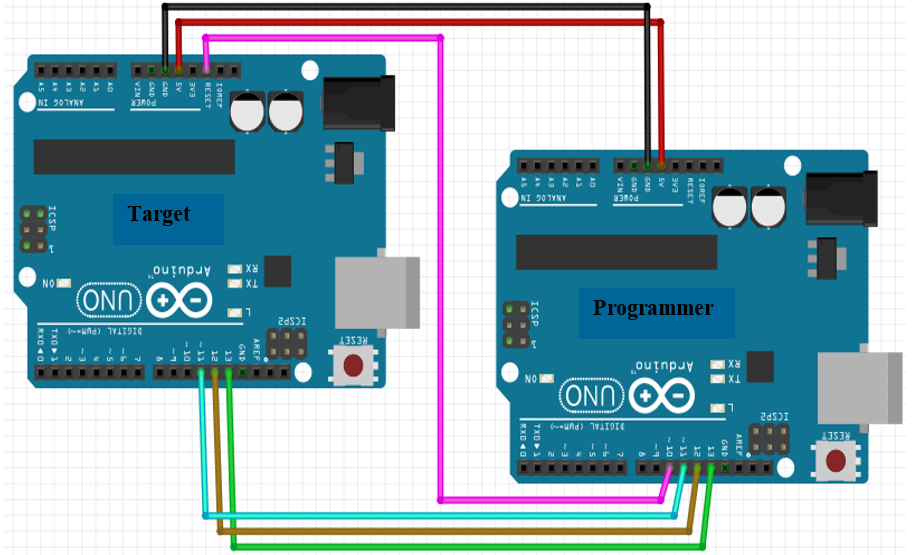
\includegraphics[scale=0.6]{EXP_26_II_Images/fig1.png}
\end{center}
\vspace{-10mm}
\begin{center} {Figure 1.Components in AWS IoT}\end{center}

\noindent \textbf{\large PROCEDURE}\\[6pt]
\textbf{A)	Simple Notification Service (SNS): Email \& message notification}\\[3pt]
The first four steps will remain the same for SNS push notification as given in fig. 1 and we are going to use the same Thing, Certificate, and Policy created in the first part. We will create a new rule for SNS push notifications.


\begin{itemize}
 \setlength\itemsep{-0.3em}
\item \textbf {Rule Creation:}\\
After login go to $ \rightarrow $ \textcolor{blue}{'IoT core'}. Click on $ \rightarrow $ \textcolor{blue}{Act} $ \rightarrow $ \textcolor{blue}{Rules}.

A new page will display, click on $ \rightarrow $ \textcolor{blue}{Create}. Provide the rule \textbf{Name} as \textbf{NotificationRule} and in the description, we can write \textbf{'Rule for sending the message'}.\par

In \textbf{ Rule query statement write :  SELECT * FROM 'outTopic' WHERE  temp $>$ 69}\par

The IoT device is publishing data on the topic- \textbf{"outTopic"} and we want notification only when the temperature exceeds 69$^{\circ}$ C.

Now Click on $ \rightarrow $ \textcolor{blue}{Add action}. A list of actions will be displayed as given in fig. 2 below.


\vspace{-5mm}
\begin{center} 
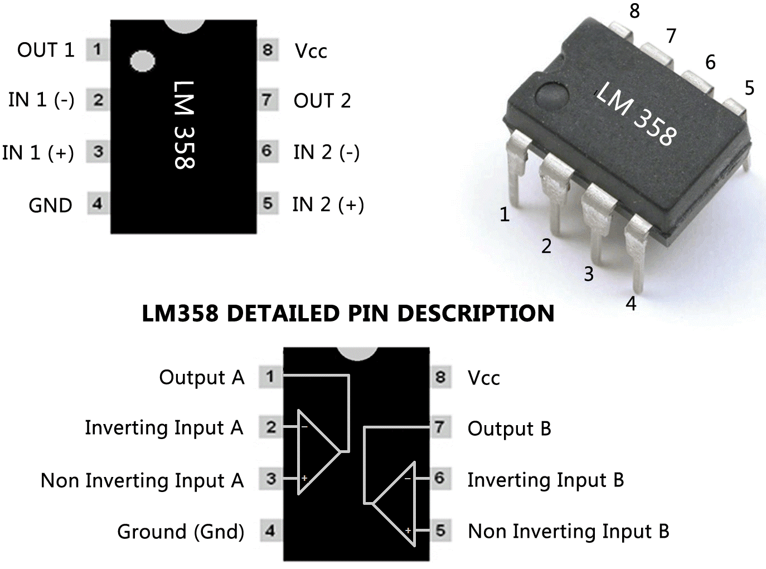
\includegraphics[scale=1]{EXP_26_II_Images/fig2.png}
\end{center}
\vspace{-10mm}
\begin{center} {Figure 2.Action list}\end{center}

\noindent Select the fourth one: \textbf{Send a message as an SNS push notification} and then click on $ \rightarrow $ \textcolor{blue}{Configure action}.
A new page as given in fig.3 below will appear. 



\vspace{-5mm}
\begin{center} 
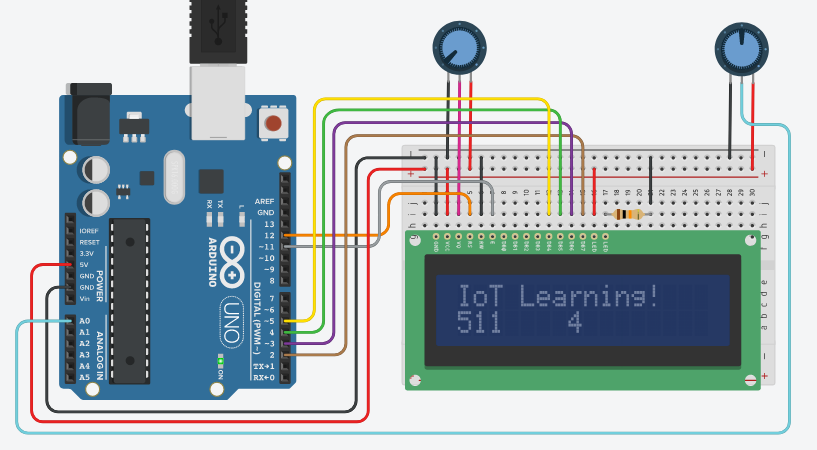
\includegraphics[scale=0.7]{EXP_26_II_Images/fig3.png}
\end{center}
\vspace{-10mm}
\begin{center} {Figure 3.Configure action }\end{center}



SNS target $ \rightarrow $ \textcolor{blue}{Create}. Provide name as \textbf{esp32alert} \& click on \textcolor{blue}{Create}\\[4pt]
Message format: Select $ \rightarrow $ RAW\\[4pt]
Click on $ \rightarrow $ \textcolor{blue}{Create Role}.\\[4pt]
Provide the name of the role say \textbf{Role4AlertMsg} and click on $ \rightarrow $ \textcolor{blue}{Create role}.\\[3pt]
\textbf{Note: Role creation is related to AWS IAM (Identity Access Management) which is an entity with permissions to make AWS service requests.}\\[4pt]
The policy will be automatically attached. Click on $ \rightarrow $ \textcolor{blue}{Add action}. \\[3pt]
Finally, click on $ \rightarrow $ \textcolor{blue}{Create rule} at the end of the page. We can see the \textbf{NotificationRule}, that we have created.\\[4pt]
\item 	\textbf{Selecting activity (what to do) when SNS receive the data}\\[4pt]
Go to AWS console $ \rightarrow $ Search for \textbf{SNS} \& click on it. Click on $ \rightarrow $ \textcolor{blue}{Topics}. Click on $ \rightarrow $ \textcolor{blue}{esp32alert}  and copy the \textcolor{blue}{ARN}.\\[4pt]
Go to the \textbf{Subscription} $ \rightarrow $ \textbf{Create subscription}. Put the copied \textbf{ARN} inside the \textbf{Topic ARN} box. Inside \textbf{Protocol box}  $ \rightarrow $ Choose \textcolor{blue}{Email}.\\[4pt]
Inside the \textbf{Endpoint box}, provide the email ad., where you want notification. \\[4pt]
Click on $ \rightarrow $ \textcolor{blue}{Create subscription}. You will get an email for confirmation, confirm subscription.\\[3pt]
Connect the ESP32 and go to the DynamoDB. Check the table Items after refreshing it. Notice the temperature, whenever it exceeds 69$^{\circ}$ C, you will get an email notification. If you have deleted the table, you can check the serial monitor and whenever the temperature exceeds  69$^{\circ}$ C, you will get an email notification. Similarly, we can have set up for SMS notification in mobile, but it is not a free trial service.

\end{itemize}

\noindent  \textbf{B)	Use Kinesis Firehose \& store data in an S3 bucket}\\
The first four steps will remain the same here as well as given in fig. 1 and we are going to use the same Thing, Certificate, and Policy created in the first part. We will create a new rule for Kinesis Firehose.

\vspace{-3mm}
\begin{itemize}
 \setlength\itemsep{-0.3em}
\item \textbf{Rule Creation:}
After login go to $ \rightarrow $ \textcolor{blue}{'IoT core'}. Click on $ \rightarrow $ \textcolor{blue}{Act} $ \rightarrow $ \textcolor{blue}{Rules}.\\[4pt]
A new page will display, click on $ \rightarrow $ Create. Provide the rule \textbf{Name} as \textbf{kinesisfirehoeRule} and in the description, we can write \textbf{Rule for sending the message}.\\[4pt]
In \textbf{Rule query statement write :  SELECT * FROM 'outTopic'} \\[4pt]
The IoT device is publishing data on the topic- \textbf{"outTopic"} and we want all fields from the data packet.\\[4pt]
 Now Click on $ \rightarrow $ \textcolor{blue}{Add action}. A list of actions will be displayed, choose \textbf{Send a message to an Amazon Kinesis Firehose stream}. Click on $ \rightarrow $ \textcolor{blue}{Configure action}.\\[6pt]
 
\item  A new page will appear and we have to create a new resource i.e. S3 bucket where Kinesis Firehose put the data. Click on $ \rightarrow $ \textcolor{blue}{Create a new resource}.\\[4pt]
A new page will appear, in the Source box choose $ \rightarrow $ \textcolor{blue}{Direct PUT} and in the \textbf{Destination} box choose $ \rightarrow $ \textcolor{blue}{Amazon S3}. The page will be expanded and the \textbf{delivery stream} name will automatically be provided. In the Destination setting, we have to create an \textbf{S3 bucket}. Click on $ \rightarrow $ \textcolor{blue}{Create}, this will take you to the S3 management console.\\[4pt]
A new pare will appear, in \textbf{General configuration} provide the Bucket \textbf{name} as \textbf{esps3bucket}. \textbf{In Object Ownership, choose} $ \rightarrow $ \textcolor{blue}{ACLs enabled}.$ \rightarrow $ \textbf{Uncheck} \textcolor{blue}{Block all public access}. Acknowledge the same by $ \rightarrow $ \textbf{ticking the small square box} below. Leave all remaining settings as default and click on $ \rightarrow $ \textcolor{blue}{Create bucket}. We can see a bucket has been created, name as \textbf{'esps3bucket'}. Go back to the Amazon Kinesis Firehose.\\[6pt]
 



\item Go to the \textbf{Destination setting} and in the \textcolor{blue}{S3 bucket} box choose $ \rightarrow $ the bucket that we have just created by \textbf{clicking} on the \textbf{Browse box}. Click on \textbf{buffer hints} $ \rightarrow $ in the \textbf{Buffer size box} put $ \rightarrow $  \textbf{1MB} and in the \textbf{Buffer interval} box put $ \rightarrow $ \textbf{180 seconds}. Leave all setting as it is and click on $ \rightarrow $ \textcolor{blue}{delivery stream}.\\[4pt]
Now go back to the \textbf{configure action page, refresh} \& in the \textbf{Choose a resource} box, choose the  resource from the drop-down menu. In the \textbf{Separator} box, choose $ \rightarrow $ \textcolor{blue}{, (comma)}.\\[4pt]
Finally, we have to create a role. Click on $ \rightarrow $ \textcolor{blue}{Create Role}. Provide \textcolor{blue}{Name} as \textcolor{blue}{KinesisFirehoseRole}. The policy will be automatically attached. Click on $ \rightarrow $ \textcolor{blue}{Add action} and finally click on $ \rightarrow $ \textcolor{blue}{Create rule}.
\end{itemize}

\noindent We can see the rule that we have created just now. Connect the IoT device and go to the $ \rightarrow $  \textbf{Amazon S3 console} and inside the  \textbf{Bucket} that we have created, we can see the new files. These new data files can be downloaded by going to the \textcolor{blue}{Action}.

\begin{center}
\textcolor{blue}{Congratulations!}\\
We have completed part-II of the experiment.
\end{center}

\noindent \textcolor{red}{Warning:} Don't keep the ESP32 powered on for a long duration. It publishes the data continuously and stores it in S3 which may cause it to cross the free limit. It is advised to delete the table after completing the experiment. This will avoid data storage in case IoT device remains on unknowingly and AWS IoT core keep connected.\par
\noindent\textbf{Keep checking the Billing Dashboard in the account section}. It will update in 24 hours and shows the charges if any along with the services that cause the charge. We can keep track of the services and associated costs. 

\noindent \textbf{\large CONCEPT DRILL}\\[6pt]
Integrate BME280 or any other sensor with ESP32 and publish the data to AWS-IoT and store it into a table in S3 bucket via Kinesis Firehose.



\end{justify}
\end{document}